% Straight up stealing preamble from Eli Holmes 
%%%%%%%%%%%%%%%%%%%%%%%%%%%%%%%%%%%%%%START PREAMBLE THAT IS THE SAME FOR ALL EXAMPLES
\documentclass{article}

%Required: You must have these
\usepackage{Sweave}
\usepackage{graphicx}
\usepackage{tabularx}
\usepackage{hyperref}

%Strongly recommended
  %put your figures in one place
 
%you'll want these for pretty captioning
\usepackage[small]{caption}

\setkeys{Gin}{width=0.8\textwidth}  %make the figs 50 perc textwidth
\setlength{\captionmargin}{30pt}
\setlength{\abovecaptionskip}{0pt}
\setlength{\belowcaptionskip}{10pt}
% manual for caption  http://www.dd.chalmers.se/latex/Docs/PDF/caption.pdf

%Optional: I like to muck with my margins and spacing in ways that LaTeX frowns on
%Here's how to do that
 \topmargin -1.5cm        
 \oddsidemargin -0.04cm   
 \evensidemargin -0.04cm  % same as oddsidemargin but for left-hand pages
 \textwidth 16.59cm
 \textheight 21.94cm 
 %\pagestyle{empty}       % Uncomment if don't want page numbers
 \parskip 7.2pt           % sets spacing between paragraphs
 %\renewcommand{\baselinestretch}{1.5} 	% Uncomment for 1.5 spacing between lines
\parindent 0pt		  % sets leading space for paragraphs
\usepackage{setspace}
%\doublespacing

%Optional: I like fancy headers
\usepackage{fancyhdr}
\pagestyle{fancy}
\fancyhead[LO]{How do climate change experiments actually change climate}
\fancyhead[RO]{2016}
 
%%%%%%%%%%%%%%%%%%%%%%%%%%%%%%%%%%%%%%END PREAMBLE THAT IS THE SAME FOR ALL EXAMPLES

%Start of the document
\begin{document}

% \SweaveOpts{concordance=TRUE}
% \bibliographystyle{/Users/Lizzie/Documents/EndnoteRelated/Bibtex/styles/nature.bst}
\title{How do climate change experiments actually change climate?} % Paper 1/Large group paper from Reconciling Experimental and Observational Approaches for Climate Change Impacts
\author{A. K. Ettinger,I. Chuine, B. Cook, J. Dukes, A. Ellison, M. Johnston, A. Panetta,\\ C. Rollinson, Y. Vitasse, E. Wolkovich}
%\date{\today}
\maketitle  %put the fancy title on
%\tableofcontents      %add a table of contents
%\clearpage
%%%%%%%%%%%%%%%%%%%%%%%%%%%%%%%%%%%%%%%%%%%%%%%%%%%

\section {Aim}

The aim is to write a Concept/Synthesis Paper about maximizing benefits of field-based climate change experiments by improved understanding of how climate is altered by these experiments. Experiments need to report what climate variables are modified by their experiment and how. This is particularly valuable for improving our understanding of biological impacts of climate change.

\section {Introduction}

\par Experimental in situ climate manipulations offer several advantages to understanding biological impacts of climate change: (controlled, relative speed- i.e. multiple manipulations can be conducted simultaneously, can hit higher temps such as those forecastest, can do them in places where other data collection is hard).
\par These advantages come at a cost, however. Experimental in situ climate
manipulations are logistically challenging, and expensive.
\par \underline{Problem:} People often want to extrapolate warming experiments to real life to understand (and forecast) biological impacts of climate change. Even in cases when this is not the explicit goal, it would be incredibly useful to be able to apply knowledge gained from these experiments to improve our understanding and forecasting of how anthropogenic warming will affect species' performance and distributions. However, our ability to make this application is limited because a detailed assessment of exactly how experimental warming treatments alter climate, and the extent to which these manipulations accurately model the real world,
is lacking.
%%%%Lizzie: I think eventually we want the tone here to acknowledge that not every experiment sets out to extrapolate to climate change, but some do -- and that really is a goal we should have. This could eventually give us an elegant way to focus in on only a couple experimental designs.
\section {Experimental climate change vs. real climate:
how do they compare?}
\subsection {Structures}
The experimental structures themselves alter temperature, in ways that are
not generally examined or reported in experimental warming studies. Compare
sham and ambient data on temperature (mixed effects models).
\begin{itemize}
\item Soil temperature is LOWER in the shams, compared with the ambient
air (Figure 1).
\item Air temperature is HIGHER in the shams, compared with the ambient
air (Figure 1).
\item The pattern was consistent for min and max air and soil temperatures, as
well (Figure 2).
\end{itemize}
\subsection {Space}
There is spatial variation in experimental warming effects, such that extrapoloation of experimental warming to forecast climate change impacts may not be a straightforward space-for-time subsitution.
\begin{itemize}
\item Analysis of plot vs. block level variation vs. treatment effects. Lizzie is working on this.
\item Documented variation in warming within plots? (This is known for open-top chambers)
\end{itemize}
\subsection {Time}
In addition, there is often temporal variation in experimental warming, and this variation may be divergent from real (i.e. non-experimental) temperature pattersn so it should carefully be considered in extrapolating experimental warming to future climate change impacts.
\begin{itemize}
\item Seasonal variations in experimental warming effects (plots over time; Christy is working on this?).
\item Daily variations in experimental warming effects (Tmin vs Tmax)
\item Compare these seasonal and daily variations to observational data (i.e. plot seasonal and daily variations for warmest vs coldest years)
\item Treatments aren’t applied consistently over the year- IR heaters can't
apply consistent warming throughout the year, and some warming experiments turn off warming during some seasons (e.g. Clark et al.).
\end{itemize}
\begin{figure}[p]
    \centering
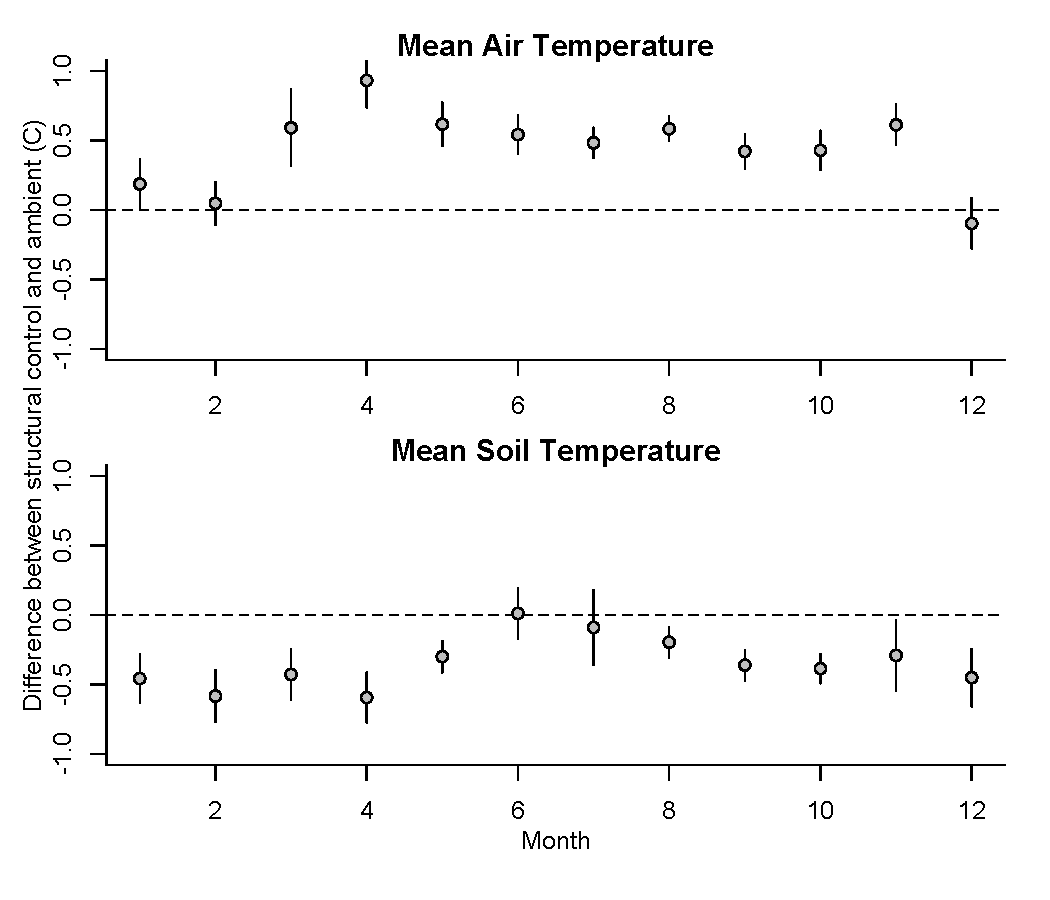
\includegraphics{Analyses/figures/ShamVSAmbient_mean.pdf}    
\caption{Difference between mean temperature in sham controls compared with ambient controls, with no sham chambers/warming infrastructure. Fixed effects from a mixed effects model are plotted in the above graph (see shamvambient.R for details). The same pattern is visible with simple box plots of ambient vs sham as well, but there are different magnitudes of differences among sites (aka studies), so i wanted to account for this statistically. Temperature data for both shams and ambient controls existed for soil in five studies, all of which are located at Harvard or Duke (clarkduke, clarkharvard,ellison,farnsworth, and marchin), and for air in only four of these studies (clarkduke, clarkharvard, ellison, and marchin). }
\end{figure}
%%%%%%%%%%
\begin{figure}[p]
    \centering
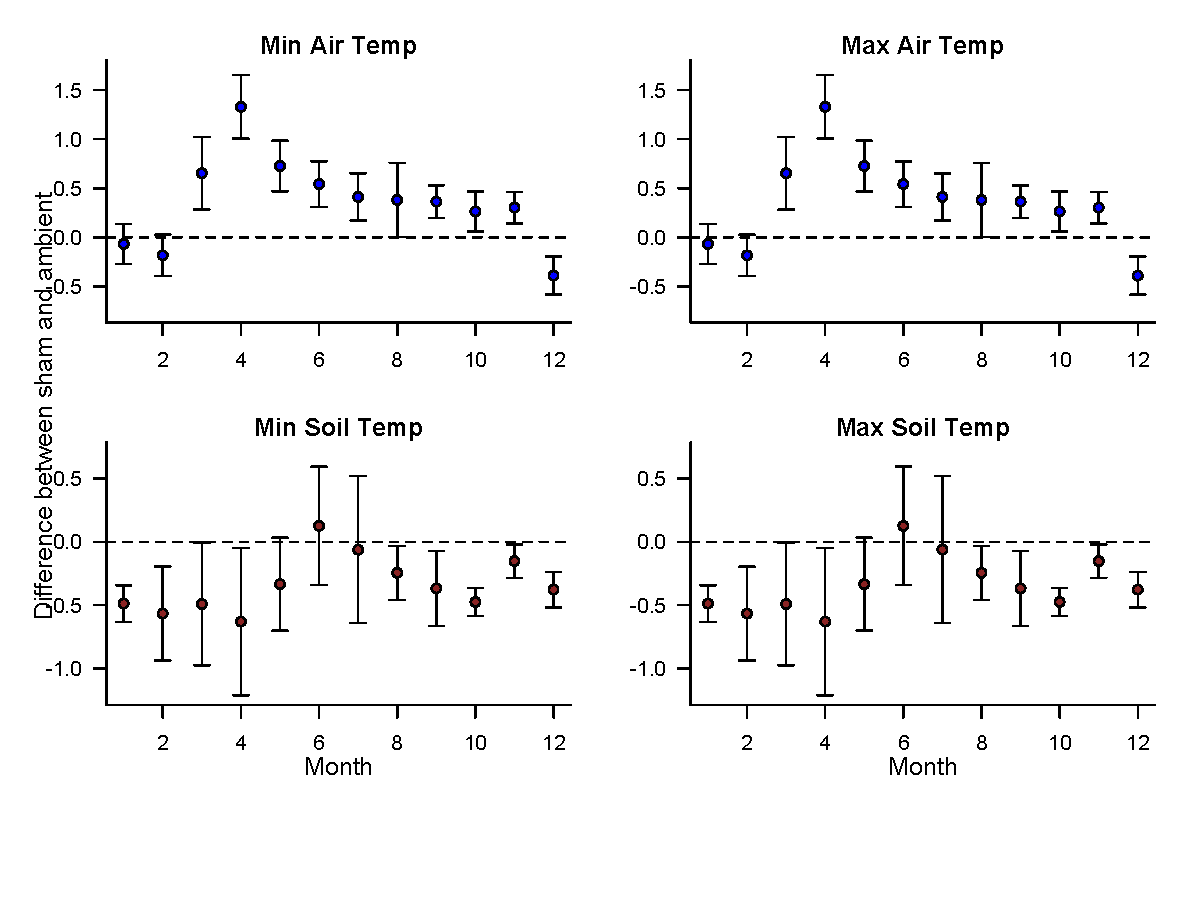
\includegraphics{Analyses/figures/ShamVSAmbient_minmax.pdf}    
\caption{Difference between min and max temperature in sham controls compared with ambient controls, with no sham chambers/warming infrastructure. Fixed effects from the a mixed effects model are plotted in the above graph (see shamvambient.R for details). }
\end{figure}
\subsection {Secondary effects of warming}
\par Temperature interacts with many other climatatic and nonclimatic factors to alterthe abiotic environment. 
\begin{itemize}
\item Effects of experimental warming on soil moisture (Figure 3, and Miriam's analysis) 
\begin{figure}[p]
    \centering
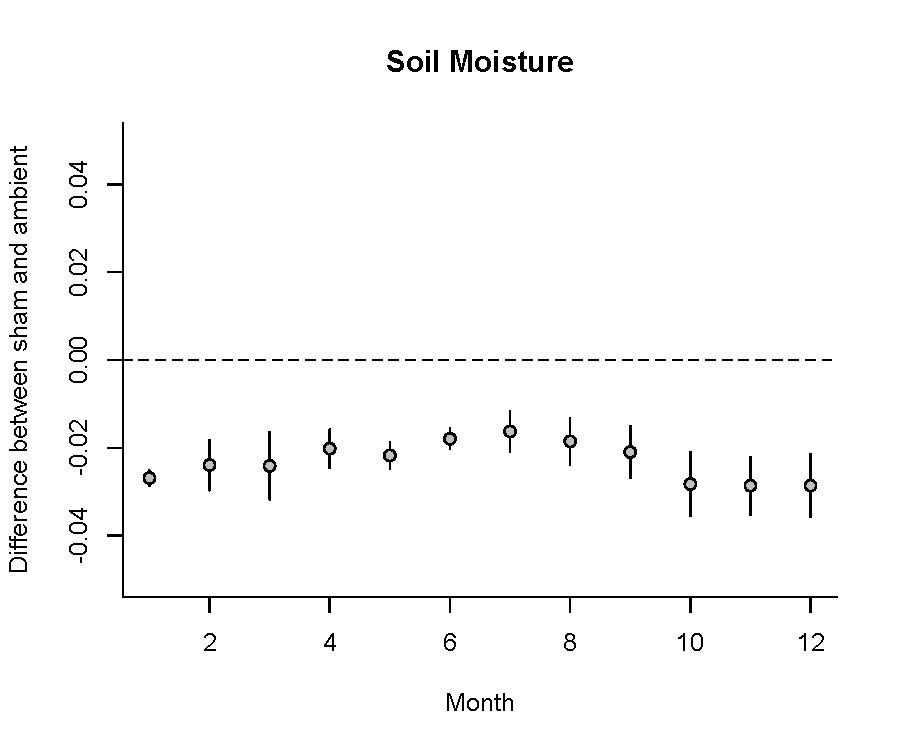
\includegraphics{Analyses/figures/ShamVSAmbient_soilmois.pdf}    
\caption{Difference between mean soil moisture in sham controls compared with ambient controls, with no sham chambers/warming infrastructure. Fixed effects from a mixed effects model are plotted in the above graph (see shamvambient.R for details). }
\end{figure}

\item Effects of experimental warming on air humidity (use Isabelle's data?).
\end{itemize}
\section {Biological Implications}
\par We have laid out several ways in which experimental warming alters more than
simply the mean temperature. We argue that these largely unintended alterations are important for scientists to fully understand and report in their research because they are likely to have biological implications. 
\par Examples:
\begin{itemize}
\item Plant phenology: likely to be altered in opposing ways by
the increased air temperatures and decrease soil moisture/temperature, cite Wolkavich et al's earlier work finding discrepency between observation and experimental phenology responses to warming.
\item Soil respiration or other microbe studies?
\item Plant growth- photosynthesis and transpiration are likely to be altered in opposing ways by the increased air temperatures and decrease soil moisture/temperature %Lizzie: I think you could find simple references in Larcher or another basic plant physiology book (Terry Chapin's?) to small temperature changes having a big effect.
\item Other ideas?
\end{itemize}
\section {Recommendations for future climate change experiments}
\par The warming effects we describe are not meant to be criticisms or to imply that experimental warming studies are not worthwhile. On the contrary, we believe that climate change experiments provide invaluable information about biological responses to warming. We also believe that we need to more fully explore the ways in which these warming experiments are altering climate, as it is clearly not simply shifting the mean. Here we describe a few recommendations to improve implementation, interpretation, and communication of future climate change experiments.
\begin{itemize}
\item Include sham and ambient controls, and collect, use, and report data collectedwithin them.
\item Carefully consider and report the timing of warming treatment applied,
including exact start and end dates within and across years.
\item Collect climate data at least twice daily, and ideally hourly; report these
data, in particular, variations in daytime and nighttime and season variations
in climate variables,
\item Report the number and cause of missing data points for climate, especially
those collected in warming treatments. For example, are data missing
because the heaters went out, or because rodents at the sensors?
\item Consider implementing and following community standards for reporting
climate data (and phenology -Chuine et al. 2017)
\item Construct regression designs to examine possible nonlinear responses to
warming
\item Publish data with good, useful metadata!
\end{itemize}

\end{document}
